\section{Hyperparameter mit Bayesian Search}

%___________________________________________________________________
\begin{frame}{Bayesian Search Erklärt}
\begin{itemize}
    \item Bayesian Search ist eine intelligente Methode zur Optimierung von Hyperparametern.
    \item Ziel: Maximierung der Validierungsgenauigkeit $f(\text{Parameter}) \rightarrow \text{Validation Accuracy}$.
    \item Idee:
        \begin{itemize}
            \item Es wird ein Modell erstellt, wie die Funktion f aussehen könnte. Es werden eingangswerte getestet, um eine aussage über das getroffene modell treffen zu können. Das modell wird angepasst. Neue paramter werte werden getestet.
            \item trade off zwischen neuen testwerten, um das modell zu verbessern und neuen testwerten, um einen neuen maximalwert zu erreichen % ist diese erklärung überhaupt richtig??????
            % \item Trade-off zwischen \textbf{Exploitation} (bekannte gute Werte) und \textbf{Exploration} (neue Werte)
            \item Probiert gezielt Parameterkombinationen, um schneller bessere Ergebnisse zu erzielen
        \end{itemize}
    \item Vorteil: Weniger Evaluierungen nötig als bei Random oder Grid Search.
\end{itemize}
\end{frame}

%___________________________________________________________________
\begin{frame}{Animation zu Bayesian Search}
\centering
\animategraphics[loop, autoplay, controls, width=\imagewidth, height=\imageheight, keepaspectratio]{0.5}{videos/frame_}{000}{006}
\imagesource{\cite{bayes_gif}}
\end{frame}

%___________________________________________________________________
\begin{frame}{Anwendung auf unser Modell}
    %  todo: zwei spalten
\begin{itemize}
    \item Anstatt zufällig Parameterkombinationen zu testen (Random Search) oder alle möglichen Kombinationen (Grid Search), wurde \textbf{Bayesian Search} verwendet.
    \item Das Modell der Funktion $\text{Validation Accuracy} = f(\text{Hyperparameter})$ wird kontinuierlich angepasst.
    \item Neue Vorschläge für Hyperparameter werden auf Basis bisheriger Ergebnisse erzeugt.
\end{itemize}

\begin{figure}
    \centering
    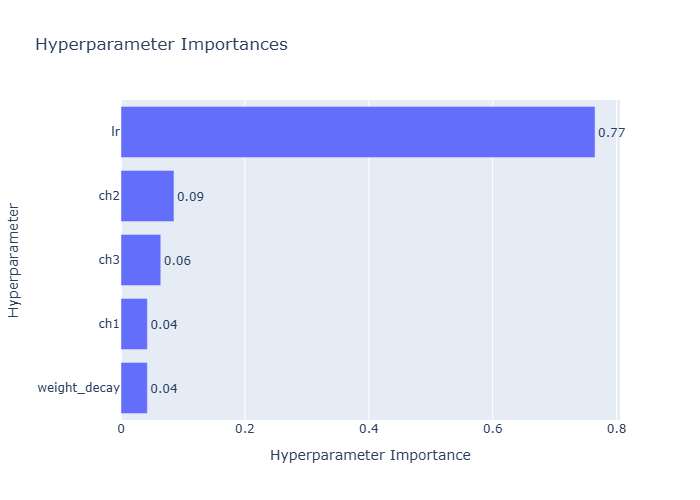
\includegraphics[width=\imagewidth, height=\imageheight, keepaspectratio]{param_importances.png}
    \caption{Relative Wichtigkeit der Hyperparameter für die Performance}
\end{figure}
\end{frame}

%___________________________________________________________________
\begin{frame}{Parameter des Bayesian Search}
\begin{itemize}
    \item \textbf{Channels:} ch1, ch2, ch3
    \item \textbf{Lernrate:} kontinuierlicher Wertebereich
    \item \textbf{Weight Decay:} kontinuierlicher Wertebereich
    \item Trials: 20
    % \item Optimierung: AdamW + Cosine Annealing Scheduler % besser nicht erwähenen
\end{itemize}
\end{frame}

%___________________________________________________________________
\begin{frame}{Bayesian Search Ergebnisse}
\begin{figure}
    \centering
    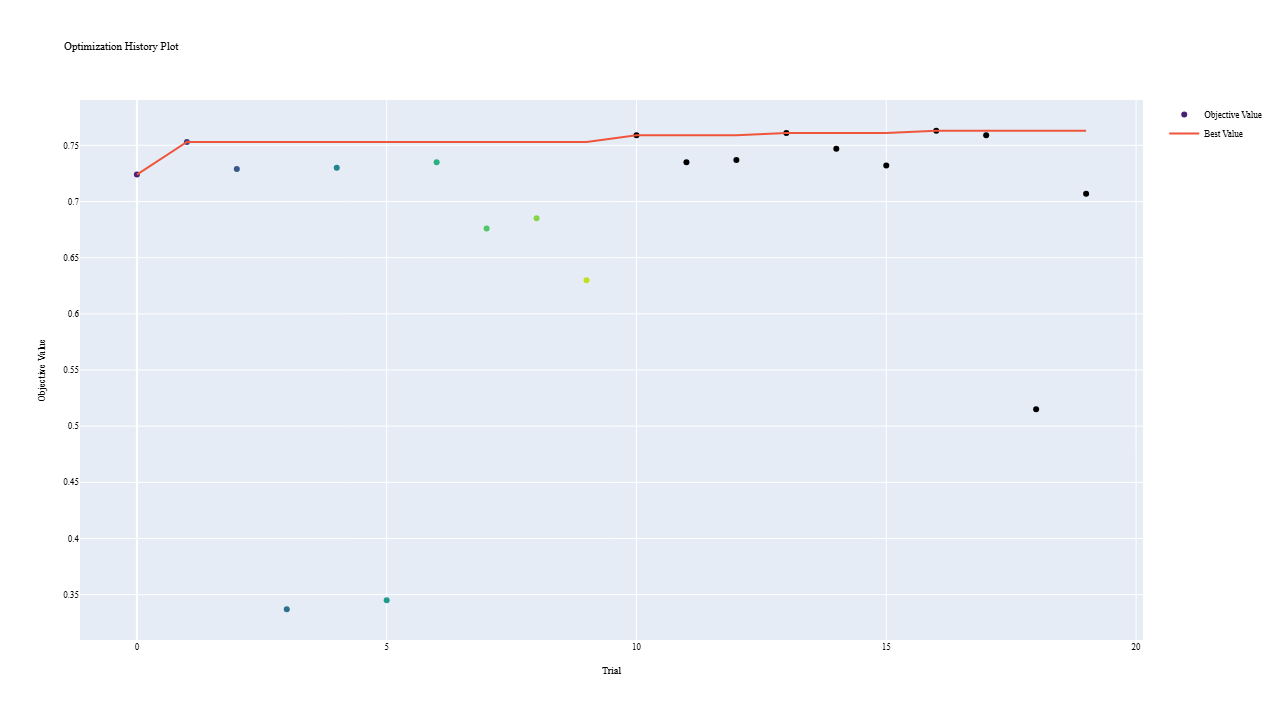
\includegraphics[width=\imagewidth, height=\imageheight, keepaspectratio]{optimization_history.png}
    \caption{Verlauf der Validierungsgenauigkeit über die Trials. Höhere Punkte = bessere Hyperparameter-Kombinationen.}
\end{figure}
\end{frame}
